\chapter{Spatial filtering}


\section{Noise}

The noise added to a pixel $p$ is defined by $n_k(p)$, 
where $k$ indicates the time step (i.e. noise changes depending on the moment the image is taken).
It is assumed that $n_k(p)$ is i.i.d and $n_k(p) \sim \mathcal{N}(0, \sigma)$.

The information of a pixel $p$ is therefore defined as:
\[ I_k(p) = \tilde{I}(p) + n_k(p) \]
where $\tilde{I}(p)$ is the real information.

\begin{description}
    \item[Temporal mean denoising] \marginnote{Temporal mean denoising}
        Averaging $N$ images taken at different time steps.
        \[ 
            \begin{split}
                O(p) &= \frac{1}{N} \sum_{k=1}^{N} I_k(p) \\
                    &= \frac{1}{N} \sum_{k=1}^{N} \Big( \tilde{I}(p) + n_k(p) \Big) \\
                    &= \frac{1}{N} \sum_{k=1}^{N} \tilde{I}(p) + \overbrace{\frac{1}{N} \sum_{k=1}^{N} n_k(p)}^{\mathclap{\text{$\mu = 0$}}} \\
                    &\approx \tilde{I}(p)
            \end{split}
        \]

        \begin{remark}
            As multiple images of the same object are required, this method is only suited for static images.
        \end{remark}

    \item[Spatial mean denoising] \marginnote{Spatial mean denoising}
        Given an image, average across neighboring pixels.

        Let $K_p$ be the pixels in a window around $p$ (included):
        \[ 
            \begin{split}
                O(p) &= \frac{1}{\vert K_p \vert} \sum_{q \in K_p} I(p) \\
                    &= \frac{1}{\vert K_p \vert} \sum_{q \in K_p} \Big( \tilde{I}(q) + n(q) \Big) \\
                    &= \frac{1}{\vert K_p \vert} \sum_{q \in K_p} \tilde{I}(q) + \frac{1}{\vert K_p \vert} \sum_{q \in K_p} n(q) \\
                    &\approx \frac{1}{\vert K_p \vert} \sum_{q \in K_p} \tilde{I}(q)
            \end{split}
        \]

        \begin{remark}
            As the average of neighboring pixels is considered, this method is only suited for uniform regions.
        \end{remark}
\end{description}



\section{Convolutions}


\subsection{Preliminaries}

\begin{description}
    \item[Convolution] \marginnote{Continuous convolution}
        Given two functions $f$ and $g$, their 1D convolution is defined as \cite{wiki:1d_convolution}:
        \[ (f * g)(t) = \int_{-\infty}^{+\infty} f(\tau)g(t - \tau) \,\text{d}\tau  \]

        In other words, at each $t$, a convolution can be interpreted as the area under $f(\tau)$ 
        weighted by $g(t - \tau)$ (i.e. $g(\tau)$ flipped w.r.t. the y-axis and with the argument shifted by $t$).

        Alternatively, it can be seen as the amount of overlap between $f(\tau)$ and $g(t - \tau)$.

        \begin{figure}[H]
            \centering
            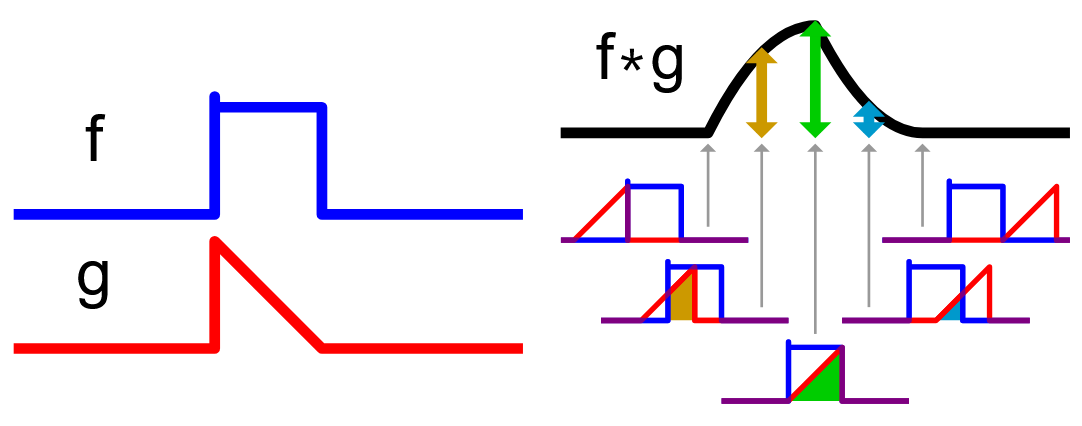
\includegraphics[width=0.4\textwidth]{./img/continuous_convolution_example.png}
            \caption{Example of convolution}
        \end{figure}

        Extended to the 2-dimensional case, the definition becomes:
        \[ (f * g)(x, y) = \int_{-\infty}^{+\infty} \int_{-\infty}^{+\infty} f(\alpha, \beta)g(x-\alpha, y-\beta) \,\text{d}\alpha\,\text{d}\beta  \]
        
        A convolution enjoys the following properties: \marginnote{Convolution properties}
        \begin{descriptionlist}
            \item[Associative] $f * (g * h) = (f * g) * h$.
            \item[Commutative] $f * g = g * f$.
            \item[Distributive w.r.t. sum] $f * (g + h) = f*g + f*h$.
            \item[Commutative with differentiation] $(f*g)' = f' * g = f * g'$
        \end{descriptionlist}

    \item[Dirac delta] \marginnote{Dirac delta}
        The Dirac delta "function" $\delta$ is defined as follows \cite{wiki:dirac,book:sonka}:
        \[ \forall x \neq 0: \delta(x) = 0 \text{, constrained to } \int_{-\infty}^{+\infty} \delta(x) \,\text{d}x = 1 \]

        Extended to the 2-dimensional case, the definition is the following:
        \[ \forall (x, y) \neq (0, 0): \delta(x, y) = 0 \text{, constrained to } \int_{-\infty}^{+\infty}\int_{-\infty}^{+\infty} \delta(x, y) \,\text{d}x\,\text{d}y = 1 \]

        \begin{description}
            \item[Sifting property] \marginnote{Sifting property}
                The following property holds:
                \[ \int_{-\infty}^{+\infty}\int_{-\infty}^{+\infty} f(x, y) \delta(\alpha-x, \beta-y) \,\text{d}x\,\text{d}y = f(\alpha, \beta) \]
                
                \begin{remark}
                    Exploiting the sifting property, the signal of an image can be expressed through an integral of Dirac deltas 
                    (i.e. a linear combination) \cite{slides:filters,book:sonka}:
                    \[ i(x, y) = \int_{-\infty}^{+\infty}\int_{-\infty}^{+\infty} i(\alpha, \beta) \delta(x-\alpha, y-\beta) \,\text{d}\alpha\,\text{d}\beta \]
                \end{remark}
        \end{description}

    \item[Kronecker delta] \marginnote{Kronecker delta}
        Discrete version of the Dirac delta \cite{wiki:kronecker}:
        \[ \delta(x) = \begin{cases}
            0 & \text{if $x \neq 0$} \\
            1 & \text{if $x = 0$} \\
        \end{cases} \]
        Extended to the 2-dimensional case, the definition is the following:
        \[ \delta(x, y) = \begin{cases}
            0 & \text{if $(x, y) \neq (0, 0)$} \\
            1 & \text{if $(x, y) = (0, 0)$} \\
        \end{cases} \]
        \begin{description}
            \item[Sifting property] \marginnote{Sifting property}
                The following property holds:
                \[ i(x, y) = \sum_{\alpha=-\infty}^{+\infty} \sum_{\beta=-\infty}^{+\infty} i(\alpha, \beta) \delta(x-\alpha, y-\beta) \]
        \end{description}
\end{description}


\subsection{Continuous convolutions}

\begin{description}
    \item[Image filter] \marginnote{Image filter}
        Operator that computes the new intensity of a pixel $p$ based on the intensities of a neighborhood of $p$.

        \begin{remark}
            Image filters are useful for denoising and sharpening operations.
        \end{remark}

    \item[Linear translation-equivariant (LTE) operator] \marginnote{LTE operator}
        A 2D operator $T\{ \cdot \}$ is denoted as:
        \[ T\{ i(x, y) \} = o(x, y) \] 
        $T\{ i(x, y) \}$ is LTE iff it is:
        \begin{descriptionlist}
            \item[Linear] 
                Given two input 2D signals $i(x, y)$, $j(x, y)$ and two constants $\alpha$, $\beta$, it holds that:
                \[ T\{ \alpha \cdot i(x, y) + \beta \cdot j(x, y) \} = \alpha T\{ i(x, y) \} + \beta T\{ j(x, y) \} \]

            \item[Translation-equivariant] 
                Given an input 2D signal $i(x, y)$ and two offsets $x_o$, $y_o$, it holds that:
                \[ \text{if } T\{ i(x, y) \} = o(x, y) \text{ then } T\{ i(x-x_o, y-y_o) \} = o(x-x_o, y-y_o) \]
        \end{descriptionlist}

        \begin{description}
            \item[Impulse response/Point spread function/Kernel] 
                Given a 2D operator $T\{ \cdot \}$, 
                its impulse response, denoted with $h$, is the output of the operator when the input signal is a Dirac delta \cite{slides:filters}:
                \[ h(x, y) \triangleq T\{ \delta(x, y) \} \]
        \end{description}
\end{description}

\begin{theorem}[LTE operators as convolutions] \marginnote{LTE operators as convolutions}
    Applying an LTE operator on an image is equivalent to computing the convolution between the image and the impulse response $h$ of the operator.
    \[ 
        \begin{split}
            T\{ i(x, y) \} &= \int_{-\infty}^{+\infty}\int_{-\infty}^{+\infty} i(\alpha, \beta) h(x-\alpha, y-\beta) \,\text{d}\alpha\,\text{d}\beta \\
                &= i(x, y) * h(x, y) 
        \end{split}
    \]
    In other words, the impulse response allows to compute the output of any input signal through a convolution.
    \begin{proof}
        Let $i(x, y)$ be an input signal and $T\{ \cdot \}$ be a 2D operator.
        We have that:
        \begin{align*}
            T\{ i(x, y) \} 
                &= T\left\{ \int_{-\infty}^{+\infty}\int_{-\infty}^{+\infty} i(\alpha, \beta) \delta(x-\alpha, y-\beta) \,\text{d}\alpha\,\text{d}\beta \right\} 
                & \text{sifting property} \\
                %
                &= \int_{-\infty}^{+\infty}\int_{-\infty}^{+\infty} T\left\{ i(\alpha, \beta) \delta(x-\alpha, y-\beta) \right\} \,\text{d}\alpha\,\text{d}\beta
                & \text{linearity of $T\{ \cdot \}$} \\
                %
                &= \int_{-\infty}^{+\infty}\int_{-\infty}^{+\infty} i(\alpha, \beta) T\left\{ \delta(x-\alpha, y-\beta) \right\} \,\text{d}\alpha\,\text{d}\beta
                & \text{linearity of $T\{ \cdot \}$} \\
                %
                &= \int_{-\infty}^{+\infty}\int_{-\infty}^{+\infty} i(\alpha, \beta) h(x-\alpha, y-\beta) \,\text{d}\alpha\,\text{d}\beta
                & \text{\small translation-equivariance of $T\{ \cdot \}$} \\
                %
                &= i(x, y) * h(x, y) 
                & \text{definition of convolution} \\
        \end{align*}  
    \end{proof}
\end{theorem}

\begin{figure}[H]
    \centering
    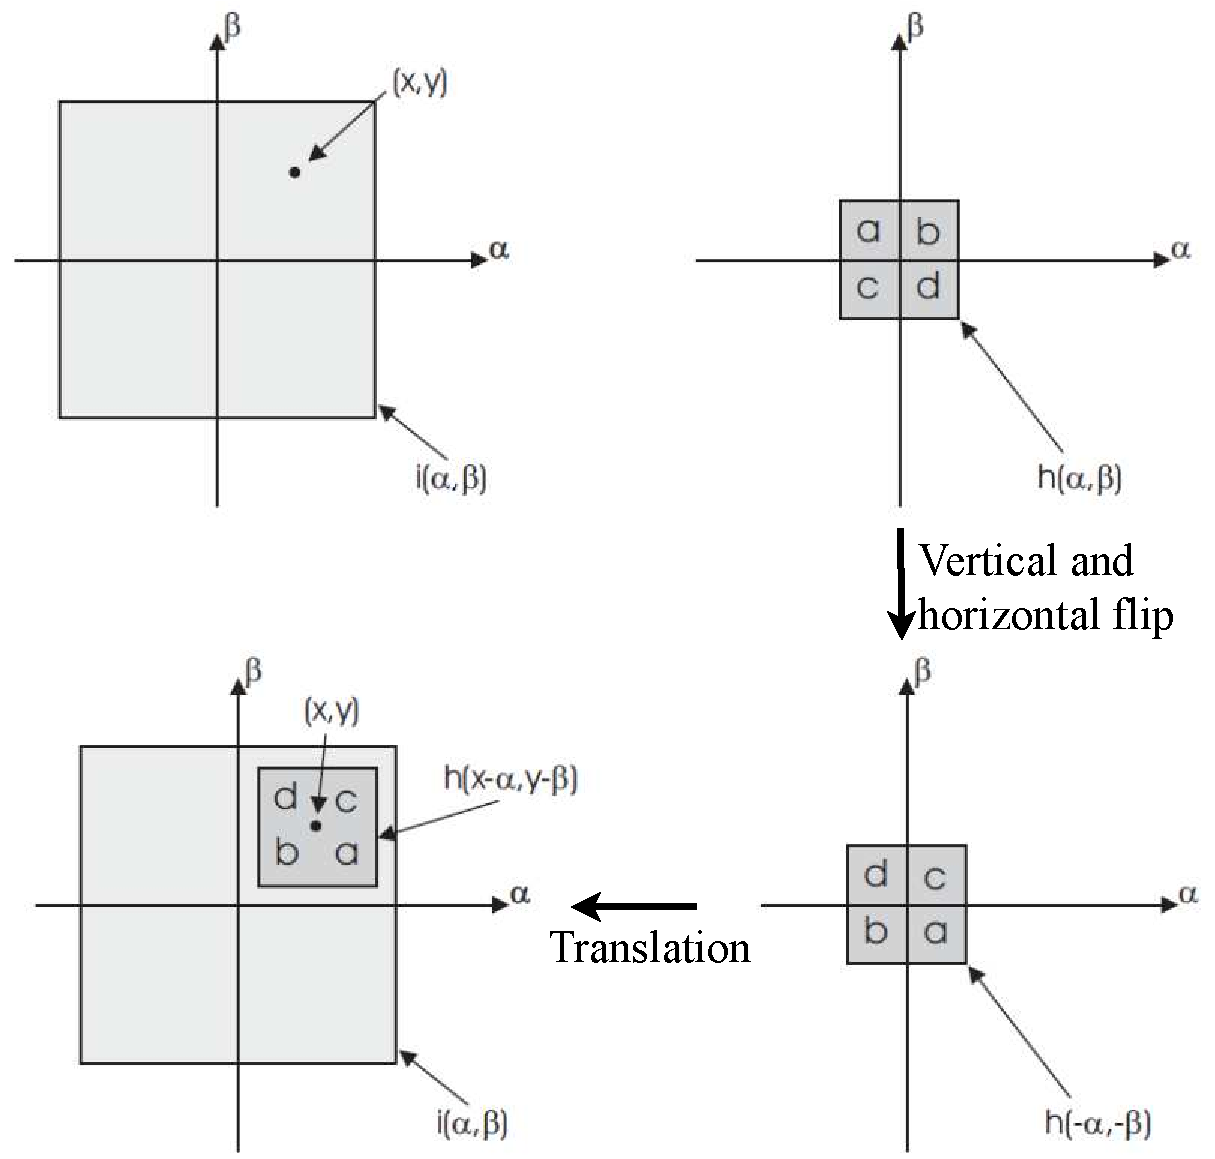
\includegraphics[width=0.4\textwidth]{./img/_convolution_graphical.pdf}
    \caption{Visualization of a convolution}
\end{figure}


\begin{description}
    \item[Cross-correlation] \marginnote{Cross-correlation}
        Given two signals $i(x, y)$ and $h(x, y)$,
        their cross-correlation computes their similarity and is defined as follows \cite{wiki:crosscorrelation}:
        \[ 
            i(x, y) \circ h(x, y) = 
            \int_{-\infty}^{+\infty}\int_{-\infty}^{+\infty} i(\alpha, \beta) h(x+\alpha, y+\beta) \,\text{d}\alpha\,\text{d}\beta =
            \int_{-\infty}^{+\infty}\int_{-\infty}^{+\infty} h(\alpha, \beta) i(\alpha-x, \beta-y) \,\text{d}\alpha\,\text{d}\beta 
        \]
        \[ 
            h(x, y) \circ i(x, y) = 
            \int_{-\infty}^{+\infty}\int_{-\infty}^{+\infty} h(\alpha, \beta) i(x+\alpha, y+\beta) \,\text{d}\alpha\,\text{d}\beta =
            \int_{-\infty}^{+\infty}\int_{-\infty}^{+\infty} i(\alpha, \beta) h(\alpha-x, \beta-y) \,\text{d}\alpha\,\text{d}\beta 
        \]

        \begin{remark}
            Cross-correlation is not commutative.
        \end{remark}

        \begin{remark}
            The cross-correlation $h \circ i$ is similar to a convolution without flipping the kernel.

            If $h$ is an even function (i.e. $h(x, y) = h(-x, -y)$), we have that $h \circ i$ has the same result of a convolution:
            \begin{align*}
                h(x, y) * i(x, y) &= \int_{-\infty}^{+\infty} \int_{-\infty}^{+\infty} i(\alpha, \beta)h(x-\alpha, y-\beta) \,\text{d}\alpha\,\text{d}\beta \\
                    &= \int_{-\infty}^{+\infty} \int_{-\infty}^{+\infty} i(\alpha, \beta)h(\alpha-x, \beta-y) \,\text{d}\alpha\,\text{d}\beta 
                    & \parbox[b]{0.25\textwidth}{\raggedleft signs in $h$ swappable for Dirac delta} \\
                    &= h(x, y) \circ i(x, y)
            \end{align*}
        \end{remark}

        \begin{figure}[H]
            \centering
            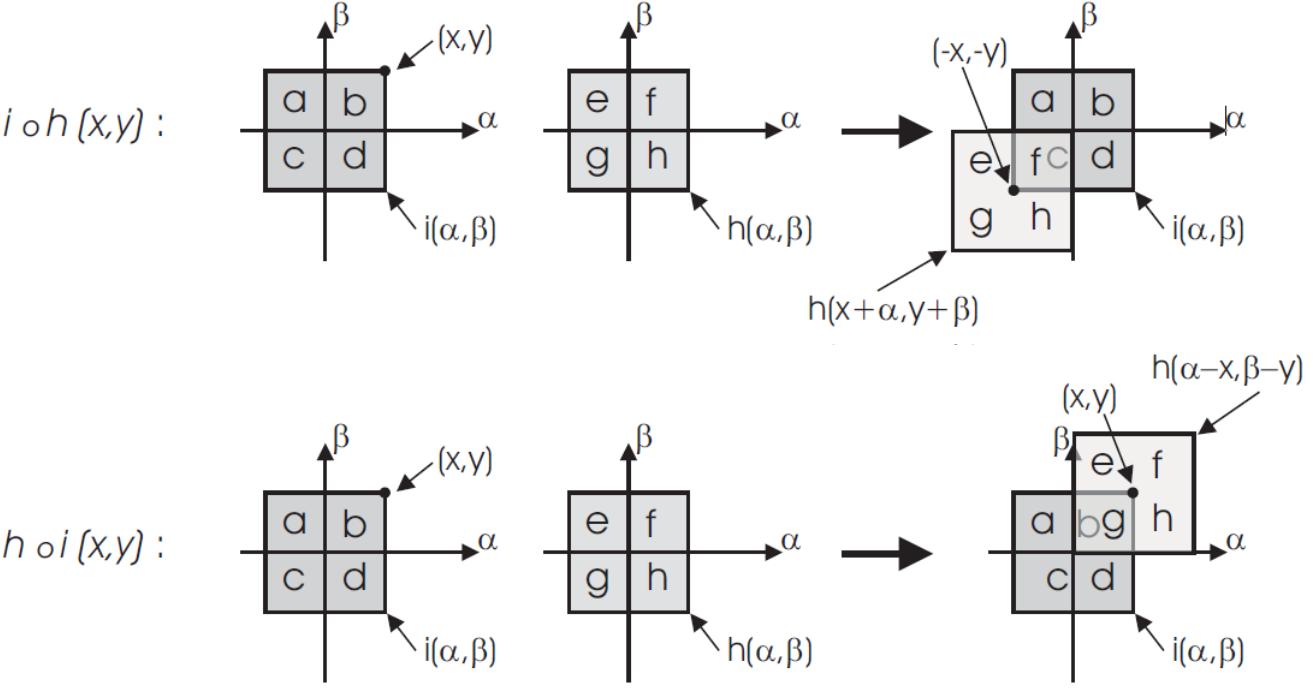
\includegraphics[width=0.6\textwidth]{./img/crosscorrelation_graphical.png}
            \caption{Visualization of cross-correlation}
        \end{figure}
\end{description}


\subsection{Discrete convolutions}

\begin{description}
    \item[Discrete convolution] \marginnote{Discrete convolution}
        Given an input 2D signal $I(i, j)$ and the kernel $H(i, j) = T\{ \delta(i, j) \}$ of a discrete LTE operator (where $\delta(i, j)$ is the Kronecker delta),
        a discrete convolution is defined as:
        \[ T\{ I(i, j) \} = \sum_{m=-\infty}^{+\infty} \sum_{n=-\infty}^{+\infty} I(m, n)H(i-m, j-n) = O(i, j) \]

        In practice, the kernel is finitely defined and is applied to each pixel of the image:
        \[ T\{ I(i, j) \} = \sum_{m=-k}^{k} \sum_{n=-k}^{k} K(m, n)I(i-m, j-n) = O(i, j) \]

        \begin{example}
            For simplicity, a kernel of size 3 is considered.
            Given an image $I$ and a kernel $K$, the output $O(1, 1)$ of the pixel $(1, 1)$ is computed as:
            \[
                \begin{split}
                    O(1, 1) &= \begin{pmatrix}
                        I(0, 0) & I(0, 1) & I(0, 2) \\
                        I(1, 0) & I(1, 1) & I(1, 2) \\
                        I(2, 0) & I(2, 1) & I(2, 2) \\
                    \end{pmatrix}
                    *
                    \begin{pmatrix}
                        K(0, 0) & K(0, 1) & K(0, 2) \\
                        K(1, 0) & K(1, 1) & K(1, 2) \\
                        K(2, 0) & K(2, 1) & K(2, 2) \\
                    \end{pmatrix} \\
                    &= I(0, 0)K(2, 2) + I(0, 1)K(2, 1) + I(0, 2)K(2, 0) + \\
                        &\,\,\,\,\,+ I(1, 0)K(1, 2) + I(1, 1)K(1, 1) + I(1, 2)K(1, 0) + \\
                        &\,\,\,\,\,+ I(2, 0)K(0, 2) + I(2, 1)K(0, 1) + I(2, 2)K(0, 0)
                \end{split}
            \] 
            Note that by definition, $K$ has to be flipped.
        \end{example}

        \begin{remark}
            In convolutional neural networks, the flip of the learned kernels can be considered implicit.
        \end{remark}
        
        \begin{description}
            \item[Border handling]  \marginnote{Border handling}
                Computing the convolution of the pixels at the borders of the image might be an issue as it goes out-of-bounds, 
                possible solutions are:
                \begin{descriptionlist}
                    \item[Crop] Ignore border pixels on which the convolution overflows.
                    \item[Pad] Add a padding to the image:
                    \begin{descriptionlist}
                        \item[Zero-padding] Add zeros (e.g. $\texttt{000}\vert a \dots d \vert\texttt{000}$).
                        \item[Replicate] Repeat the bordering pixel (e.g. $\texttt{aaa}\vert a \dots d \vert\texttt{ddd}$).
                        \item[Reflect] Use the $n$ pixels closest to the border (e.g. $\texttt{cba}\vert abc \dots dfg \vert\texttt{gfd}$).
                        \item[Reflect\_101] Use the $n$ pixels closest to the border, skipping the first/last one (e.g. $\texttt{dcb}\vert abcd \dots efgh \vert\texttt{gfe}$).
                    \end{descriptionlist}
                \end{descriptionlist}
        \end{description}
    \end{description}


\subsection{Common linear kernels}

\begin{description}
    \item[Mean filter] \marginnote{Mean filter}
        LTE operator that computes the intensity of a pixel as the average intensity of the pixels in its neighborhood.

        The kernel has the form (example with a $3 \times 3$ kernel):
        \[
            \begin{pmatrix}
                \frac{1}{9} & \frac{1}{9} & \frac{1}{9} \\
                \frac{1}{9} & \frac{1}{9} & \frac{1}{9} \\
                \frac{1}{9} & \frac{1}{9} & \frac{1}{9} \\
            \end{pmatrix} 
            = 
            \frac{1}{9} \begin{pmatrix}
                1 & 1 & 1 \\
                1 & 1 & 1 \\
                1 & 1 & 1 \\
            \end{pmatrix} 
        \]

        \begin{remark}
            The mean filter has a low-pass effect which allows the removal of details from the signal.
            This allows for image smoothing and, to some extent, denoising (but adds blur).
        \end{remark}
        \begin{remark}
            As the intensity of a pixel is computed by averaging its neighborhood, 
            the results for pixels located between low-intensity and high-intensity areas might not be ideal.
        \end{remark}

        \begin{figure}[H]
            \centering
            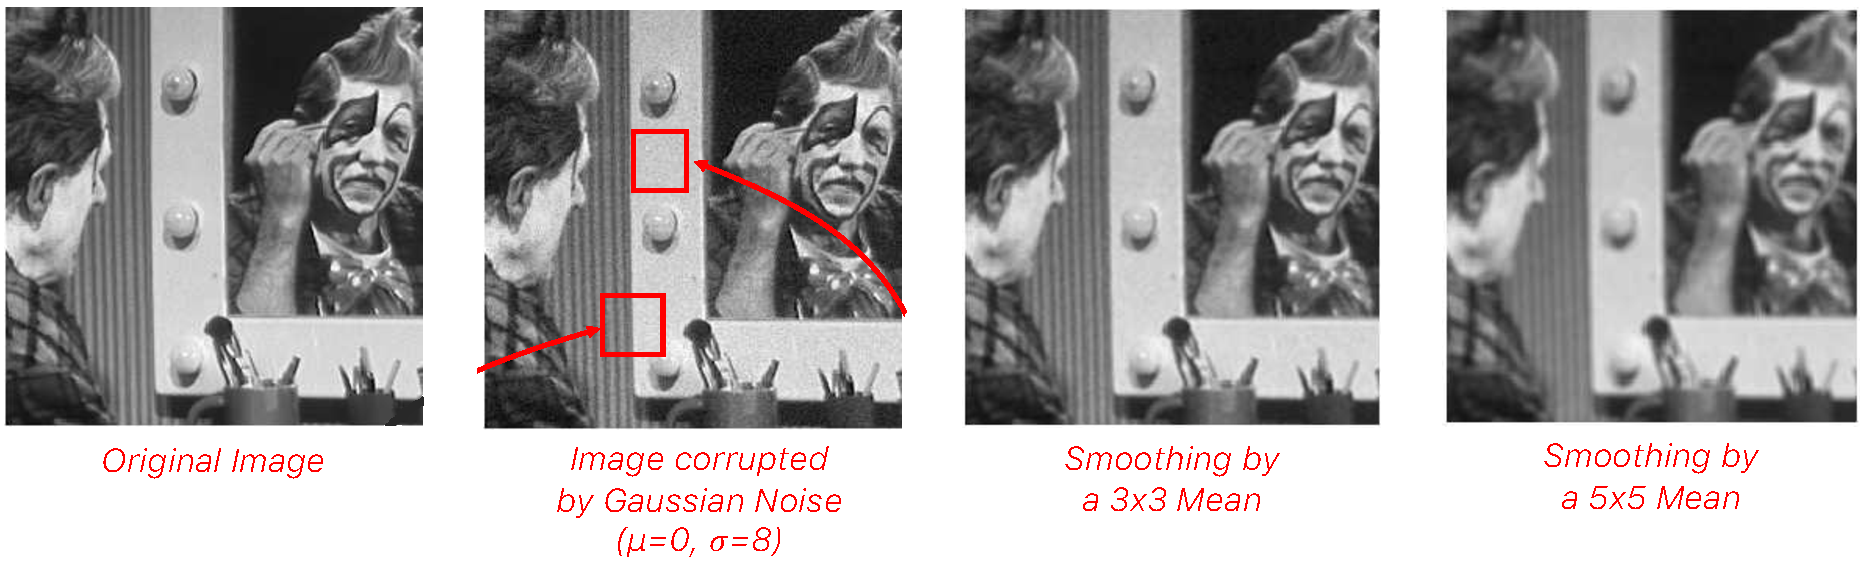
\includegraphics[width=0.85\textwidth]{./img/_mean_filter_example.pdf}
            \caption{Example of mean filter application}
        \end{figure}

    \item[Gaussian filter] \marginnote{Gaussian filter}
        LTE operator whose kernel follows a 2D Gaussian distribution with $\mu=0$ and given $\sigma$.

        \begin{remark}
            The smoothing strength of the filter grows with $\sigma$.
        \end{remark}

        \begin{figure}[H]
            \centering
            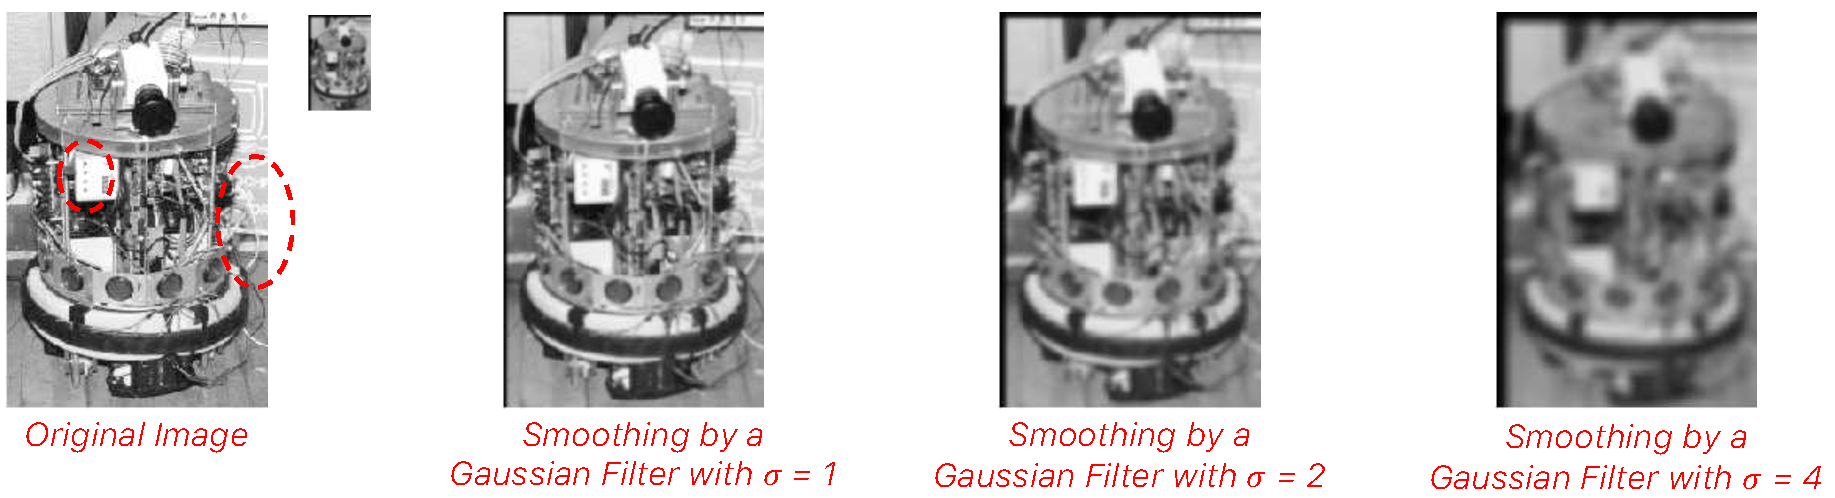
\includegraphics[width=0.85\textwidth]{./img/_gaussian_filter_example.pdf}
            \caption{Example of Gaussian filter application}
        \end{figure}

        \begin{description}
            \item[Sampling]
                In practice, the kernel is created by sampling from the wanted Gaussian distribution.
                One can notice that a higher $\sigma$ results in a more spread distribution and therefore a larger kernel is more suited,
                on the other hand, a smaller $\sigma$ can be represented using a smaller kernel as it is more concentrated around the origin.

                As a rule-of-thumb, given $\sigma$, an ideal kernel is of size $(2\lceil 3\sigma \rceil + 1) \times (2\lceil 3\sigma \rceil + 1)$.

            \item[Separability]
                As a 2D Gaussian $G(x, y)$ can be decomposed into a product of two 1D Gaussians $G(x, y) = G_1(x)G_2(y)$,
                it is possible to split the convolution into two 1D convolutions.
                \[ 
                    \begin{split}
                        I(x, y) * G(x, y) &= \int_{-\infty}^{+\infty}\int_{-\infty}^{+\infty} I(\alpha, \beta) G(x-\alpha, y-\beta) \,\text{d}\alpha\,\text{d}\beta \\
                            &= \int_{-\infty}^{+\infty}\int_{-\infty}^{+\infty} I(\alpha, \beta) G_1(x-\alpha)G_2(y-\beta) \,\text{d}\alpha\,\text{d}\beta \\
                            &= \int_{-\infty}^{+\infty} G_2(y-\beta) \left( \int_{-\infty}^{+\infty} I(\alpha, \beta) G_1(x-\alpha) \,\text{d}\alpha \right) \,\text{d}\beta \\
                            &= (I(x, y) * G_1(x)) * G_2(y)
                    \end{split}
                \]

                \begin{remark}
                    The speed-up in number-of-operations is linear.
                \end{remark}
        \end{description}
\end{description}


\subsection{Common non-linear kernels}

\begin{remark}
    Linear filters are ineffective when dealing with impulse noise and 
    have the side effect of blurring the image.

    \begin{figure}[H]
        \centering
        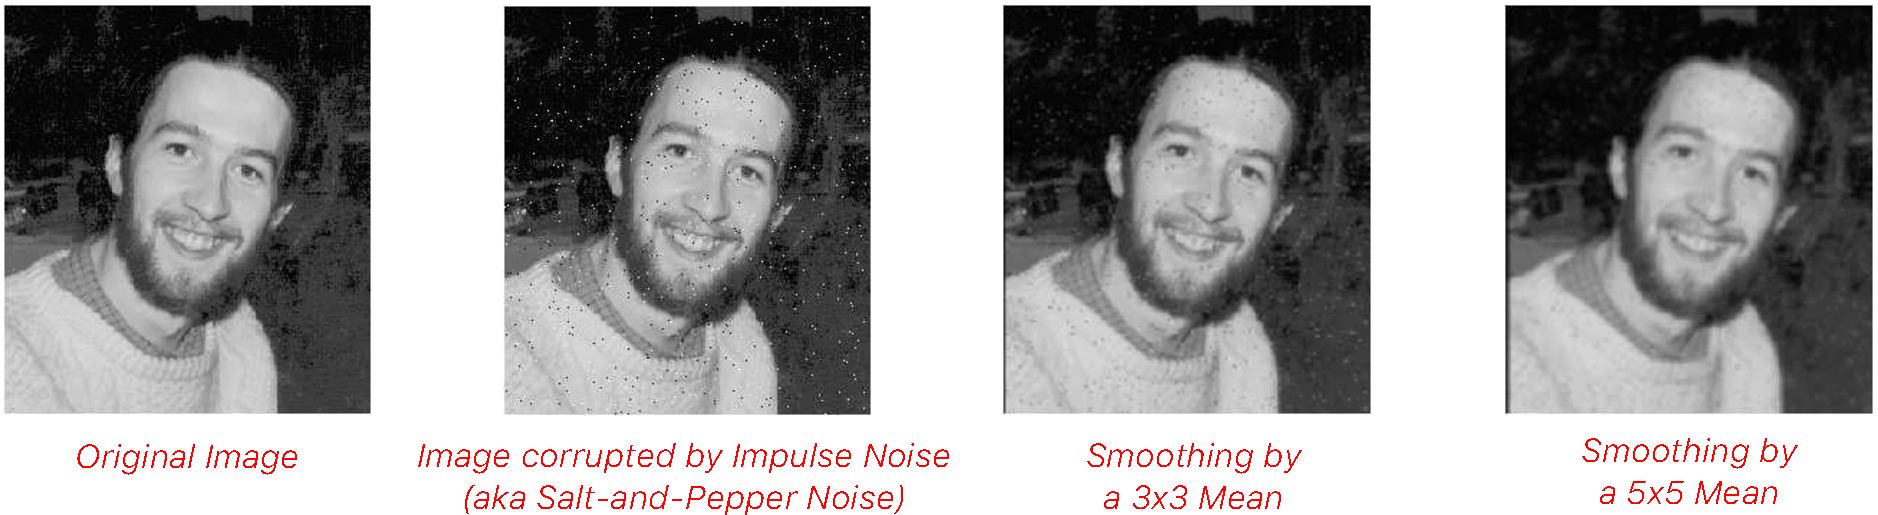
\includegraphics[width=0.85\textwidth]{./img/_impulse_noise_example.pdf}
        \caption{Example of impulse noise and denoising with mean filter}
    \end{figure}
\end{remark}

\begin{remark}
    As they lose linearity, non-linear filters are technically not convolutions anymore.
\end{remark}

\begin{description}
    \item[Median filter] \marginnote{Median filter}
        The intensity of a pixel is obtained as the median intensity of its neighborhood.

        \begin{remark}
            Median filters are effective in removing impulse noise (as outliers are excluded) without introducing significant blur.
            It also tends to result in sharper edges.
        \end{remark}

        \begin{remark}
            Median filters are not suited for Gaussian noise.
            It might be useful to apply a linear filter after a median filter.
        \end{remark}

        \begin{figure}[H]
            \centering
            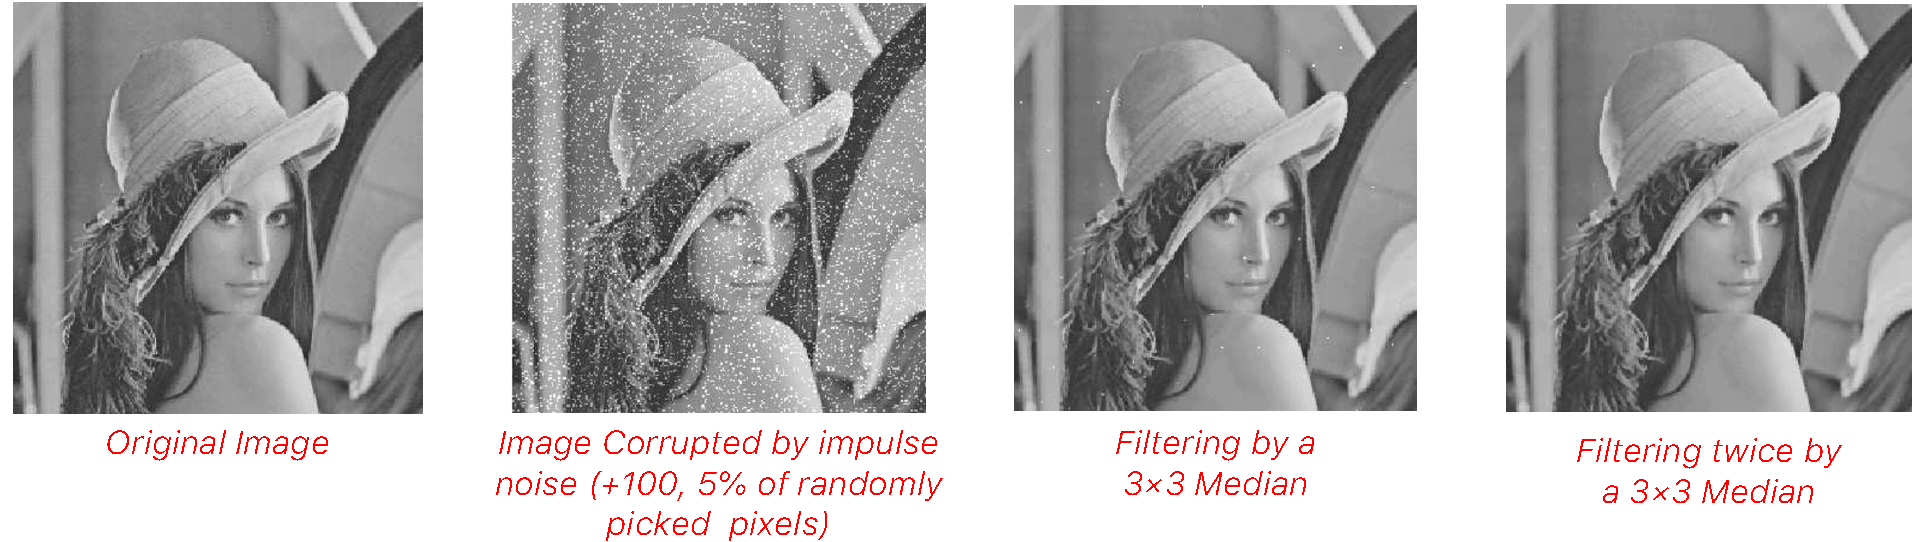
\includegraphics[width=0.85\textwidth]{./img/_median_filter_example.pdf}
            \caption{Example of median filter application}
        \end{figure}


    \item[Bilateral filter] \marginnote{Bilateral filter}
        Given two pixels $p$ and $q$, the following can be computed:
        \begin{descriptionlist}
            \item[Spatial distance] $d_s(p, q) = \Vert p - q \Vert_2$
            \item[Range/intensity distance] $d_r(p, q) = \vert \texttt{intensity}(p) - \texttt{intensity}(q) \vert$
        \end{descriptionlist}

        Given a pixel $p$, its neighborhood $\mathcal{N}(p)$ and the variances $\sigma_s$, $\sigma_r$ of two Gaussians,
        the bilateral filter applied on $p$ is computes as follows:
        \[ 
            \begin{split}
                O(p) &= \sum_{q \in \mathcal{N}(p)} H(p, q) \cdot \texttt{intensity}(q) \\
                &\text{where } H(p, q) = \frac{G_{\sigma_s}(d_s(p, q)) G_{\sigma_r}(d_r(p, q))}{\sum_{z \in \mathcal{N}(p)} G_{\sigma_s}(d_s(p, z)) G_{\sigma_r}(d_r(p, z))}
            \end{split}    
        \]
        where the denominator of $H$ is a normalization factor.

        \begin{remark}
            Bilateral filters allow to deal with Gaussian noise without the introduction of blur.
        \end{remark}

        \begin{remark}
            Neighboring pixels with similar intensities result in larger weights in the filter,
            while pixels with different intensities (i.e. near an edge) result in smaller weights.
            This allows to effectively ignore pixels that belong to a different object from being considered when computing the intensity of a pixel.
        \end{remark}

        \begin{figure}[H]
            \centering
            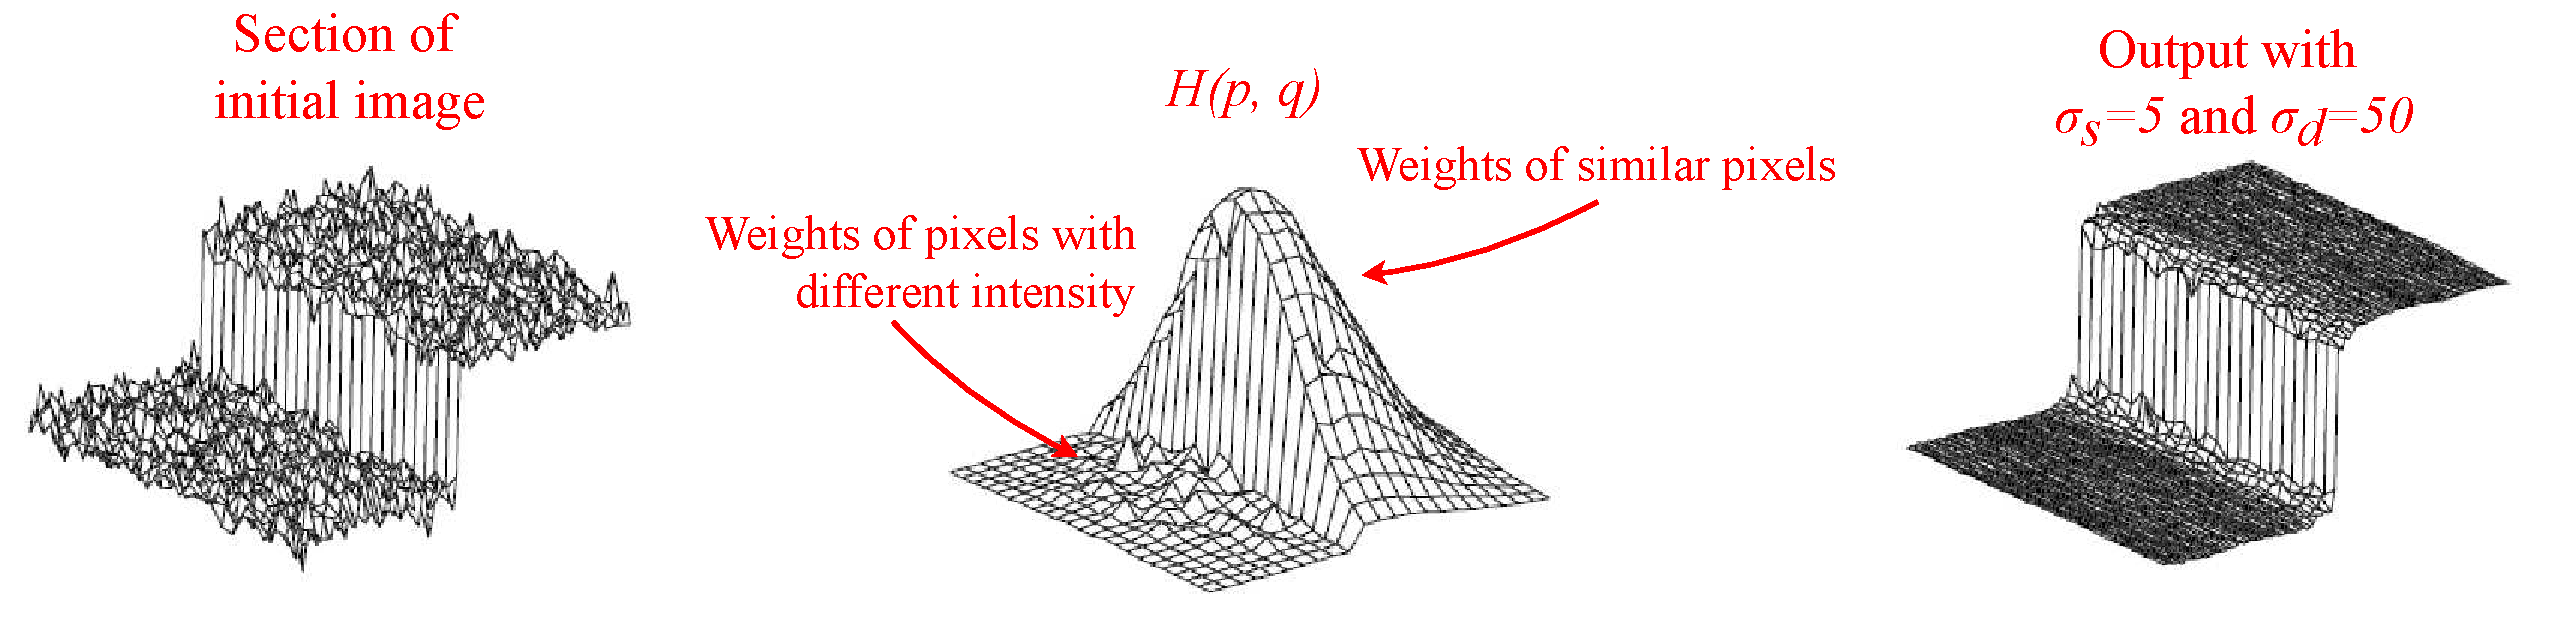
\includegraphics[width=0.9\textwidth]{./img/_bilateral_filter_example.pdf}
            \caption{Example of bilateral filter application}
        \end{figure}

    
    \item[Non-local means filter] \marginnote{Non-local means filter}
        Exploits patches with similar pixels to denoise the image.

        \begin{minipage}{0.75\textwidth}
            Let:
            \begin{itemize}
                \item $I$ be the image plane.
                \item $\mathcal{N}_i$ be the intensity matrix of a patch centered on the pixel $i$.
                \item $S_i$ be a neighborhood of the pixel $i$.
                \item $h$ be the bandwidth (a hyperparameter).
            \end{itemize}
            The intensity of a pixel $p$ is computed as follows:
            \[
                \begin{split}
                    O(p) &= \sum_{q \in S_p} w(p, q) \cdot \texttt{intensity}(q) \\
                    \text{where }& w(p, q) = \frac{1}{Z(p)} e^{-\frac{\Vert \mathcal{N}_p - \mathcal{N}_q \Vert_2^2}{h^2}} \\
                                & Z(p) = \sum_{q \in I} e^{\frac{\Vert \mathcal{N}_p - \mathcal{N}_q \Vert_2^2}{h^2}}
                \end{split}
            \]
        \end{minipage}
        \begin{minipage}{0.25\textwidth}
            \centering
            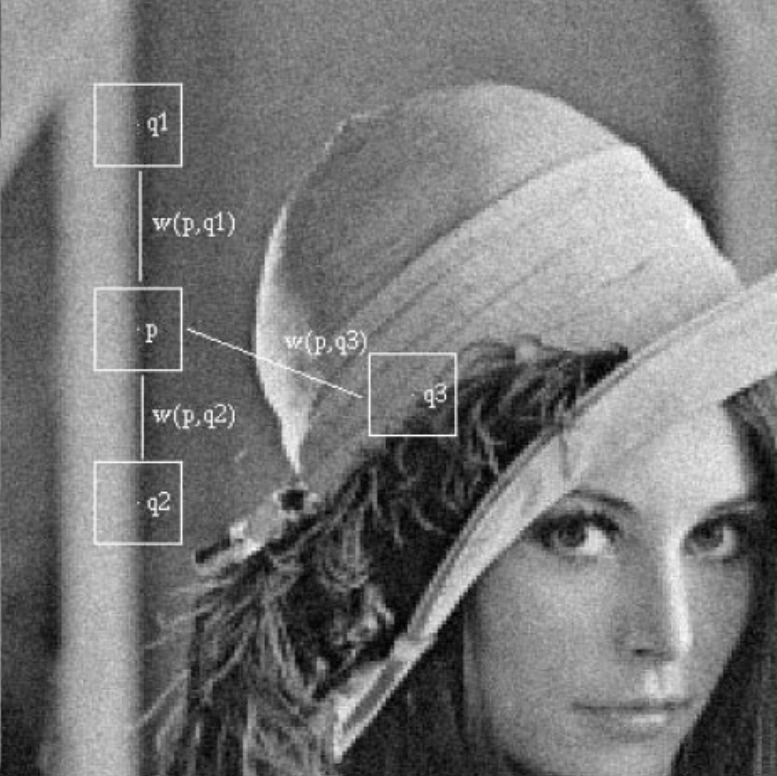
\includegraphics[width=\linewidth]{./img/non_local_means_filter.png}
        \end{minipage}

        Instead of using the full image plane $I$, a neighborhood $S_p$ is used for computational purposes.
        $Z(p)$ is a normalization factor.
\end{description}